\documentclass[11pt,letterpaper]{article}
\usepackage[lmargin=1in,rmargin=1in,tmargin=1in,bmargin=1in]{geometry}
\usepackage{../style/homework}
\usepackage{../style/commands}
\setbool{quotetype}{false} % True: Side; False: Under
\setbool{hideans}{false} % Student: True; Instructor: False

% -------------------
% Content
% -------------------
\begin{document}

\homework{17: Due 12/01}{There is no branch of mathematics, however abstract, which may not some day be applied to phenomena of the real world.}{Nikolai Lobachevsky}

% Problem 1
\problem{10} Showing all your work and as accurately as possible, plot the region given by the inequalities below:
	\[
	\begin{aligned}
	x_1 + &x_2 \leq 5 \\
	x_1 &\leq 3 \\
	x_1, & \, x_2 \geq 0 \\
	\end{aligned}
	\]
Is the region bounded or unbounded?
	\[
	\fbox{
	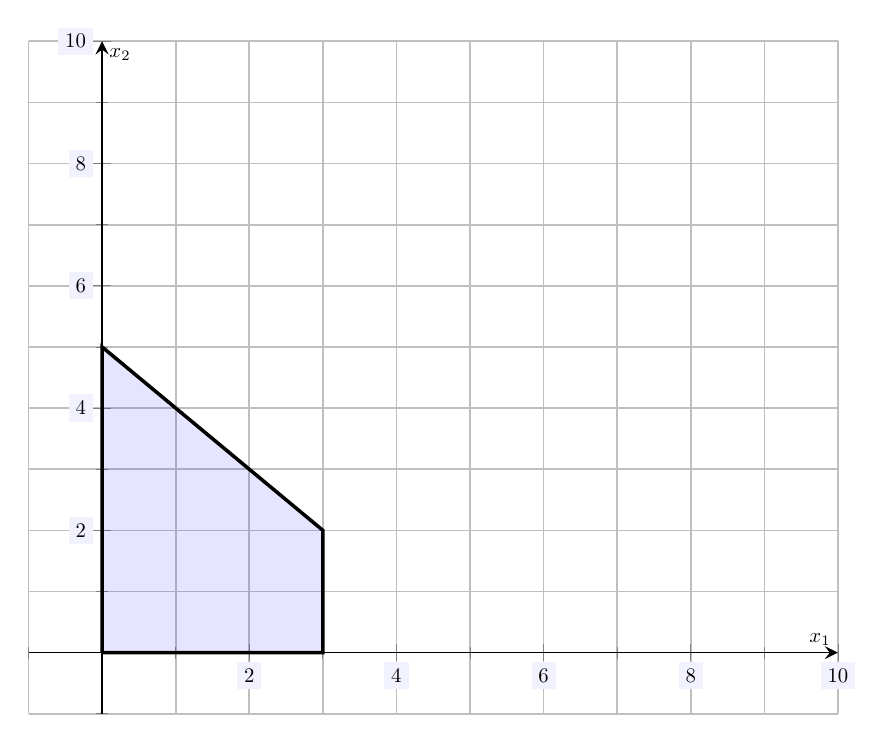
\begin{tikzpicture}[scale=1.5,every node/.style={scale=0.5}]
	\begin{axis}[
	grid=both,
	axis lines=middle,
	ticklabel style={fill=blue!5!white},
	xmin= -1, xmax=10,
	ymin= -1, ymax=10,
	xtick={0,2,4,6,8,10},
	ytick={0,2,4,6,8,10},
	minor tick = {-1,0,1,...,10},
	xlabel=\(x_1\),ylabel=\(x_2\),
	]
%	\addplot[domain= -1:10, line width=0.03cm] (x,5-x);
%	\draw[line width=0.03cm] (3,-10.5) -- (3,10.5);
	\draw[line width=0.01cm,fill= blue,opacity=0.1] (0,0) -- (0,5) -- (3,2) -- (3,0) -- (0,0);
	\draw[line width=0.03cm] (0,0) -- (0,5) -- (3,2) -- (3,0) -- (0,0);
	\end{axis}
	\end{tikzpicture}
	}
	\] \pspace

\sol First, observe that if we `solve' $x_1 + x_2 \leq 5$ for $x_2$, we obtain $x_2 \leq 5 - x_1$. The line $x_2= 5 - x_1$ is a line with $y$-intercept $(0, 5)$ and slope $-1$. Because $x_2 \leq 5 - x_1$, we need shade below this line. The line $x_1= 3$ is a vertical line with $x_1= 3$ for all points on the line. Because $x_1 \leq 3$, we need shade to the left of this line. The line $x_1= 0$ is the $y$-axis. Because $x_1 \geq 0$, we need shade to the right of the $y$-axis. The line $x_2= 0$ is the $x$-axis. Because $x_2 \geq 0$, we need shade above the $x$-axis. [Note: Together, the inequalities $x_1, x_2 \geq 0$ simply state that the region must be in Quadrant~I.] Clearly, we need find the intersection of the lines $x_2= 5 - x_1$ and $x_1= 3$. But if $x_1= 3$, then $x_2= 5 - x_1= 5 - 3= 2$. Therefore, these intersect at the point $(x_1, x_2)= (3, 2)$. Combining all this data gives the region shaded above. \pspace

Because we can clearly draw a `ball' around this region, e.g. the circle at the origin with radius 10, the region is bounded. 



\newpage



% Problem 2
\problem{10} Showing all your work and as accurately as possible, plot the region given by the inequalities below:
	\[
	\begin{aligned}
	x_1 + 2x_2 &\geq 7 \\
	x_1 + x_2 &\geq 5 \\
	x_1, x_2 &\geq 0
	\end{aligned}
	\]
Is the region bounded or unbounded?
	\[
	\fbox{
	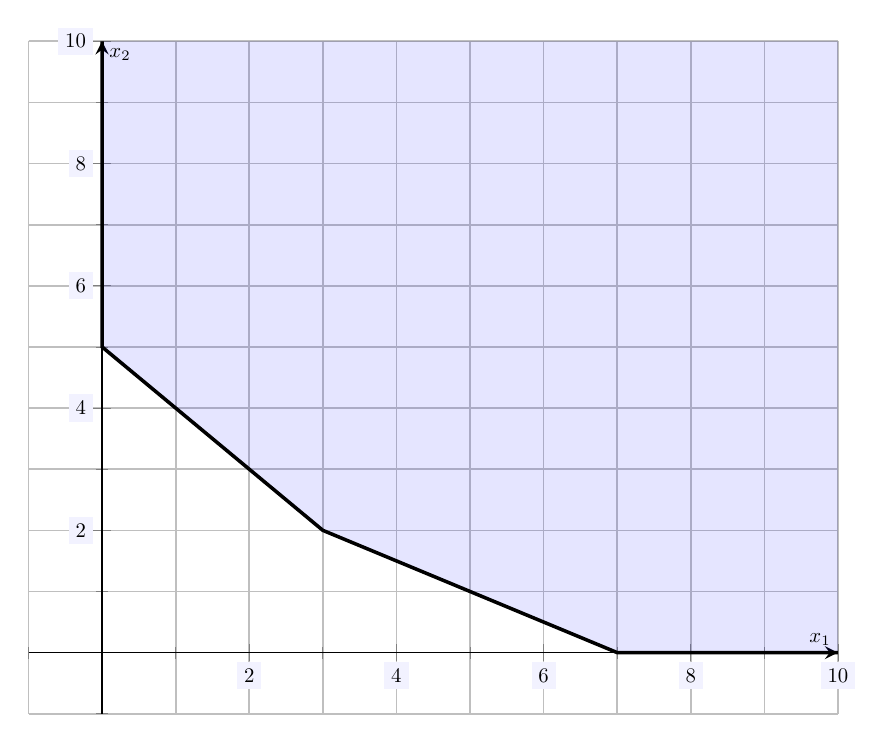
\begin{tikzpicture}[scale=1.5,every node/.style={scale=0.5}]
	\begin{axis}[
	grid=both,
	axis lines=middle,
	ticklabel style={fill=blue!5!white},
	xmin= -1, xmax=10,
	ymin= -1, ymax=10,
	xtick={0,2,4,6,8,10},
	ytick={0,2,4,6,8,10},
	minor tick = {-1,0,1,...,10},
	xlabel=\(x_1\),ylabel=\(x_2\),
	]
%	\addplot[line width= 0.03cm, domain= -2:10] (x, 5-x);
%	\addplot[line width= 0.03cm, domain= -2:10] (x, 7/2 - 1/2*x);
	\draw[line width=0.01cm,fill= blue,opacity=0.1] (0,10) -- (0,5) -- (3,2) -- (7, 0) -- (10,0) -- (10,10) -- (0,10);
	\draw[line width=0.03cm] (0,10) -- (0,5) -- (3,2) -- (7, 0) -- (10,0);
	\end{axis}
	\end{tikzpicture}
	}
	\] \pspace

\sol First, observe that if we `solve' $x_1 + 2x_2 \geq 7$ for $x_2$, we obtain $x_2 \geq \frac{7}{2} - \frac{1}{2}\, x_1$. The line $x_2= \frac{7}{2} - \frac{1}{2}\,x_1$ has $y$-intercept $\frac{7}{2}$ and slope $-\frac{1}{2}$. Because $x_2 \geq \frac{7}{2} - \frac{1}{2}\,x_1$, we need shade above this line. `Solving' $x_1 + x_2 \geq 5$ for $x_2$, we obtain $x_2 \geq 5 - x_1$. The line $x_2= 5 - x_1$ has $y$-intercept 5 and slope $-1$. Because $x_2 \geq 5 - x_1$, we need shade above this line. The line $x_1= 0$ is the $y$-axis. Because $x_1 \geq 0$, we need shade to the right of the $y$-axis. The line $x_2= 0$ is the $x$-axis. Because $x_2 \geq 0$, we need shade above the $x$-axis. [Note: Together, the inequalities $x_1, x_2 \geq 0$ simply state that the region must be in Quadrant~I.] Sketching these lines, we clearly need find the intersection of $x_2= \frac{7}{2} - \frac{1}{2}\,x_1$ and $x_2= 5 - x_1$. But then we have $\frac{7}{2} - \frac{1}{2}\, x_1= 5 - x_1$. Multiplying both sides by 2, we obtain $7 - x_1= 10 - 2x_1$. But then we have $7 + x_1= 10$ so that $x_1= 3$. Using this in the line $x_2= 5 - x_1$, we have $x_2= 5 - 3= 2$. Therefore, the intersection of $x_2= \frac{7}{2} - \frac{1}{2}\,x_1$ and $x_2= 5 - x_1$ is $(3, 2)$. Clearly, we also need the $x$-intercept of $x_2= \frac{7}{2} - \frac{1}{2}\,x_1$. At the $x$-intercept, $x_2= 0$. But then $0 = \frac{7}{2} - \frac{1}{2}\,x_1$ so that $\frac{1}{2}\,x_1= \frac{7}{2}$. This implies that $x_1= 7$. Therefore, the line $x_2= \frac{7}{2} - \frac{1}{2}\,x_1$ has $x$-intercept $(7, 0)$. Combining all this information gives the region shaded above. \pspace

Because there are points, $(x, y)$ with arbitrarily large coordinates, the region is unbounded. That is, there is no `ball' of fixed size which can enclose the region. Therefore, the region is unbounded. 


\end{document}